\chapter{Solution Idea} \label{chap:solutionideas}

This section presents our plan for obtaining the objectives discussed in section \ref{chap:intro}. 
In our approach, we propose a Model-based and Data-driven development approach using the LEAN development approach. As mentioned earlier, LEAN contains three phases Build, Measure, and Learn.

In the Build phase, we plan to create the \texttt{(1) UI Prototyping} using the drag and drop approach, \texttt{(2) Model} these prototypes, and create \texttt{(3) Experiments and Tasks} from the models and assign them to the users.
In the Measure phase, we plan to measure the \texttt{(4) Experiment and the Task measurements}.
Finally, in the Learn phase, we would analyze the results from the \texttt{(5) Experiments and the Tasks}, \texttt{(6) Tune our model and modify the product}.  

Consider an example of a \textbf{``A video streaming service''} called \texttt{VideoStreamer (VS)}.
As shown in figure \ref{solutionideas:fig:stakeholders}, this company has different stakeholders. 
We divide them into two groups the developers (e.g., programmers, designers, etc.) and the non-developers (e.g., product owners) to improve the product.
\begin{figure}
    \centering
    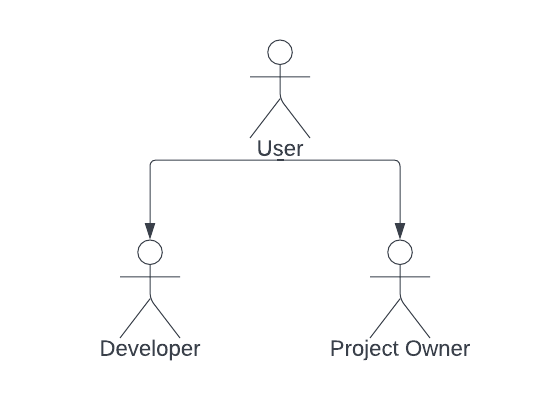
\includegraphics[scale=0.2]{images/solution-ideas/Stakeholder.png}
    \caption{Different Stakeholders in the Company VS}
    \label{solutionideas:fig:stakeholders}
\end{figure}
Usually, the developers are responsible for developing various features required for the company. 
But, the problem is, in the beginning, knowing which design fits better for a UI is impossible. 
Therefore, we need to perform experiments on the UI using A/B testing.
So, the developers develop different variants for experimenting with the UI and get feedback from the non-developers.
This feedback process wastes a lot of time, so our solution is to give freedom to the product owners and reduce the gap between the product owners and the developers by allowing the product owners to create the UI using UI prototyping.

\section{Build}
\subsection{Visualising the Prototypes} 

We plan to implement the UI prototyping in a low-code technique for our solution because it needs negligible installation, setup, training, and implementation work. 
The low-code technique enables the rapid creation and deployment of business applications with the least amount of coding effort. 
We plan to create a system for non-developers to modify the UI elements in a canvas-like structure in an application. 
For this, the product owners first create a canvas screen and input the name for that screen. 
As shown in figure \ref{solutionideas:fig:uiprototyping}, they can add UI elements like buttons, input buttons, select buttons, etc., on the canvas screen. 
We propose to use angular\footnote{Angular: \url{https://angular.io/}} for developing the application. 
Various UI elements are available for the drag and drop of the UI elements, as shown in figure \ref{solutionideas:fig:uiprototyping} (right side).

\begin{figure}[h]
    \centering
    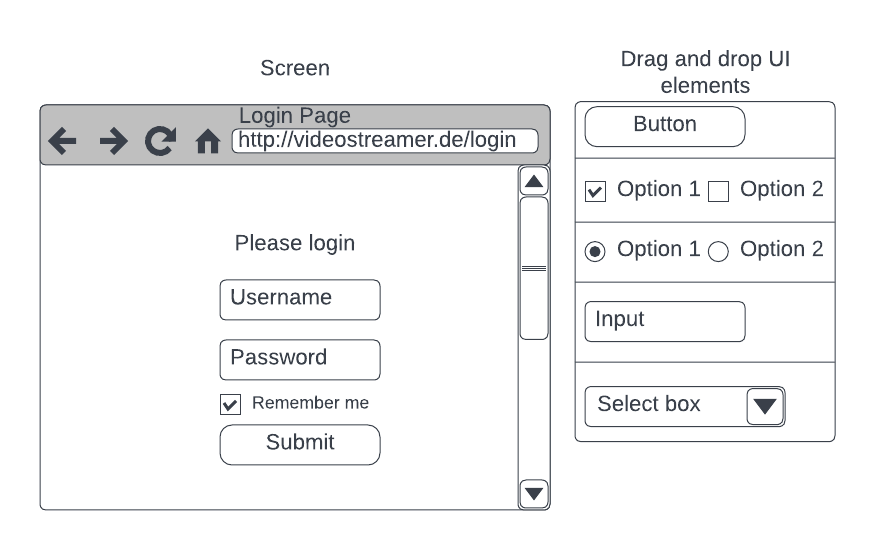
\includegraphics[scale=0.4]{images/solution-ideas/UIPrototyping.png}
    \caption{UI Prototyping using drag and drop of UI elements}
    \label{solutionideas:fig:uiprototyping}
\end{figure}

Once the non-developers finalize the UI screen, they can move to the next screen by some logic (E.g., clicking on a button to go to the next screen). 
This way, the non-developers can design the entire application, having a sequence flow (i.e., the user will register, go to the Login page, next to the Dashboard page, etc.), using the canvas screen, and adjust the UI elements. 
This way, the non-developers can build the entire application quickly without any programming knowledge. 

\subsection{Modelling the Prototypes}

\begin{figure}[h]
	\centering
  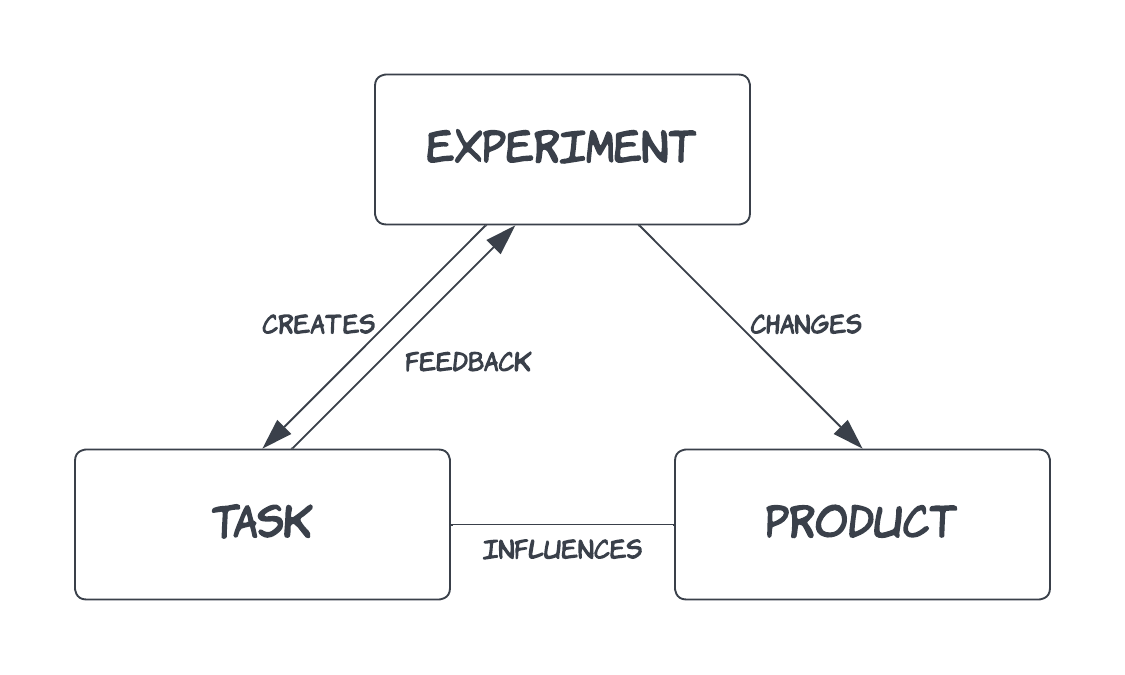
\includegraphics[width=0.7\textwidth]{images/solution-ideas/Triangle.png}
	\caption{Triangle of Experiment, Task, and Product}
	\label{solutionideas:fig:triangle}
\end{figure}

In our application, we plan to convert the screens the non-developers develop into models. 
To do that, we need a modeling language that fits our requirements. 
Based on our domain, we need models for \texttt{Experiments}, \texttt{Tasks} and \texttt{Product}.

\paragraph{Experiment:} In the \texttt{Experiment Model}, we store different properties of the UI elements along with the variant information.\\
E.g., from \texttt{Videostreamer app}: If the experiment is on a \texttt{Button} element, our model should have information about the position of the button, the style of the button (storing the color, font, etc.), the title of the button, etc. All this information would be stored in the model as its properties or attributes.
The Model also stores information of different variants of a particular application screen. (E.g., see figure \ref{solutionideas:fig:experimentingvariants} the Grid and the List View)
Moreover, the model can obtain this information from the UI prototyping done by non-developers using the drag-and-drop feature.

\paragraph{Product:} In the \texttt{Product Model}, we store information about the product and all its components as independent parts.
This model stores all the different screens available in a software application and links them.\\
E.g., from \texttt{Videostreamer app}: A video streamer would have different screens (see Fig \ref{solutionideas:fig:metamodel} right side), a Home screen, a Video search screen, a Video display screen, etc. 
These screens are modeled to relate different screens and the elements within a specific screen. 
We plan to create Meta-models  (see Fig \ref{solutionideas:fig:metamodel} left side) and develop relationships between them. 
Moreover, the models should be able to accept measurements (e.g., \texttt{ClickRate} to measure the user clicks, \texttt{ViewTime} to measure the time spent by the user) to determine the best fit among the variants.

\paragraph{Task:} In the \texttt{Task Model}, we store a sequence of activities that the user needs to perform and obtain feedback as measurements from the users for testing the software product.\\
E.g., from \texttt{Videostreamer app}: We would give a task to a user U1, saying ``Navigate to the movie M1'' and measure the number of steps/clicks and the time required for the user to perform this task.

There are some relationships between these models as depicted by the figure \ref{solutionideas:fig:triangle} \\ 
\texttt{(1) Experiment-Task, (2) Experiment-Product, and (3) Task-Product} relationships.

\paragraph{Experiment-Task:} An experiment can create various tasks for the users and get some feedback in the form of data from the Task model. 

\paragraph{Experiment-Product:} From an experiment, it can be decided which is the best variant for a product and can thus modify and improve the product in an iteratively continuous process.

\paragraph{Task-Product:} A task should be created based on the current state of the product, and thus it creates a relationship between the task and the product.

\begin{figure}[bt]
	\centering
  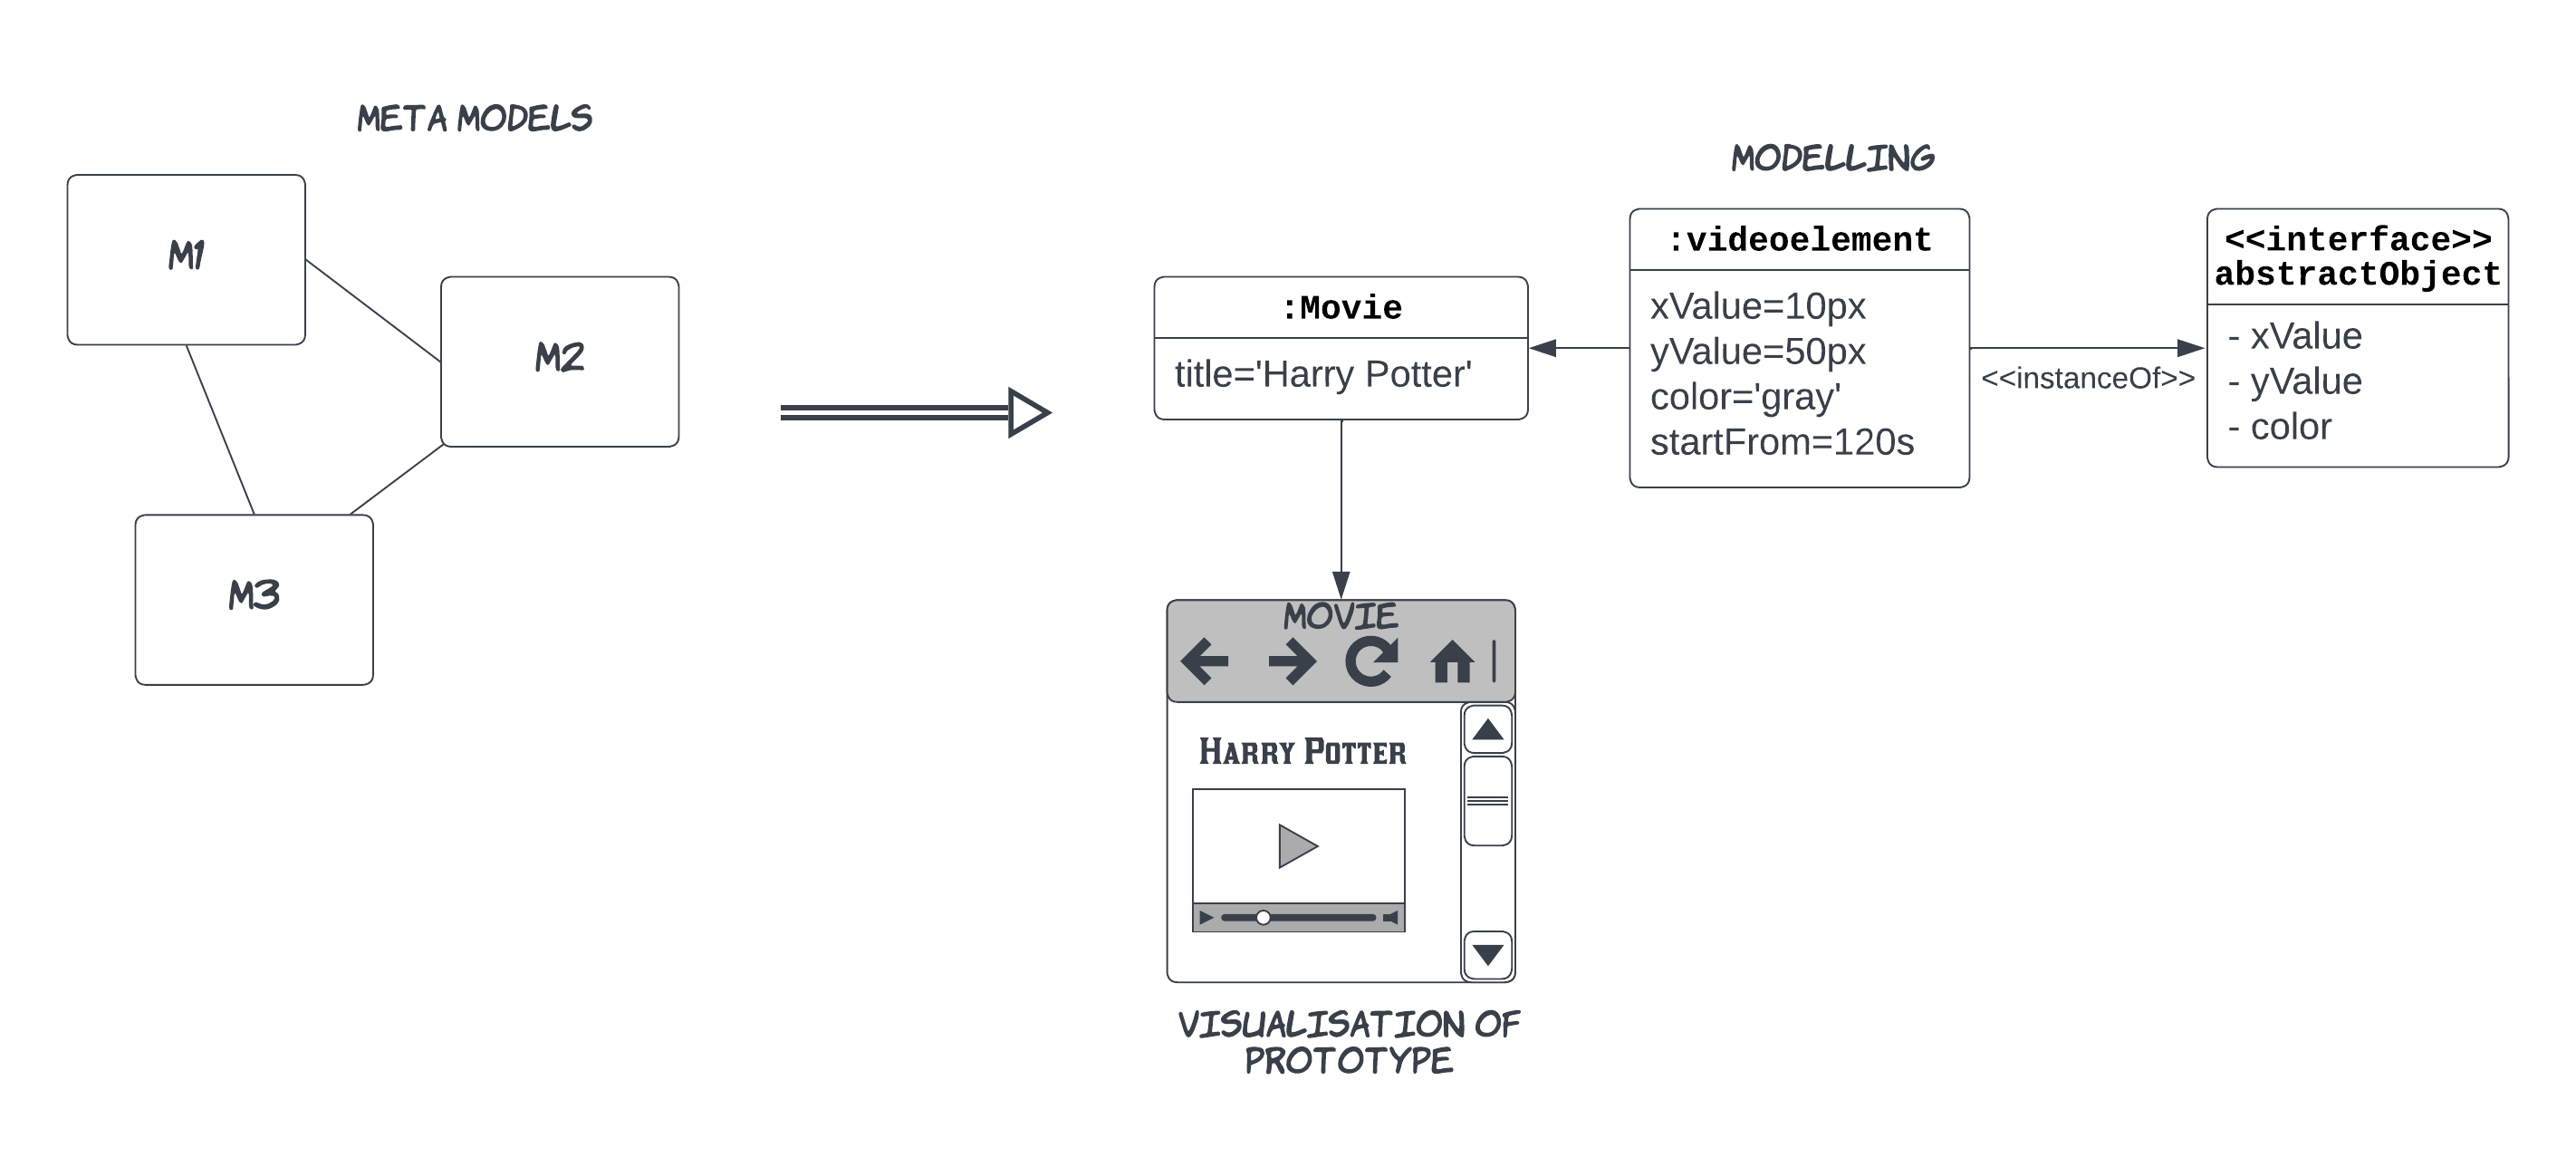
\includegraphics[width=1.05\textwidth]{images/solution-ideas/MetaModel.png}
	\caption{Example Meta Model}
	\label{solutionideas:fig:metamodel}
\end{figure}
\subsection{Experimenting using A/B Testing}

The product owners continuously investigate new features and product enhancement opportunities by conducting frequent experiments. 
The owners better understand their customers' experiences by creating that feedback loop with users. 
As a result, they can constantly give practical solutions. 
There are various types of experimenting\footnote{A/B Testing: \url{https://www.hotjar.com/conversion-rate-optimization/glossary/ab-testing/}} options available for the product owners.
In our solution, we try to find which of these better fit our requirements and find an approach for conducting experiments with the UI elements. 
The product owner should be able to create various experiments by moving the UI elements and having multiple views for a particular screen. \\ \\
E.g., from our \texttt{Videostreamer app}: As shown in figure \ref{solutionideas:fig:experimentingvariants}, the experiment model can create different variants for the component \texttt{View}: the \texttt{Grid view} (on the left) and the \texttt{List view} (on the right). 
These experiments are conducted on the users by dividing the users into groups and assigning one of the variants to a group. 
This type of setup is called the ``\texttt{Between-group}'' design experiment. 
Then, the users would be given specific tasks per the \texttt{Task Model}, and the measurements will provide feedback to the \texttt{Experiment Model}. 
The data obtained are analyzed (explained in section \ref{solutionideas:section:dataanalysis}), and finally, we find the best variant for a product's component. 

\begin{figure}[ht]
	\centering
  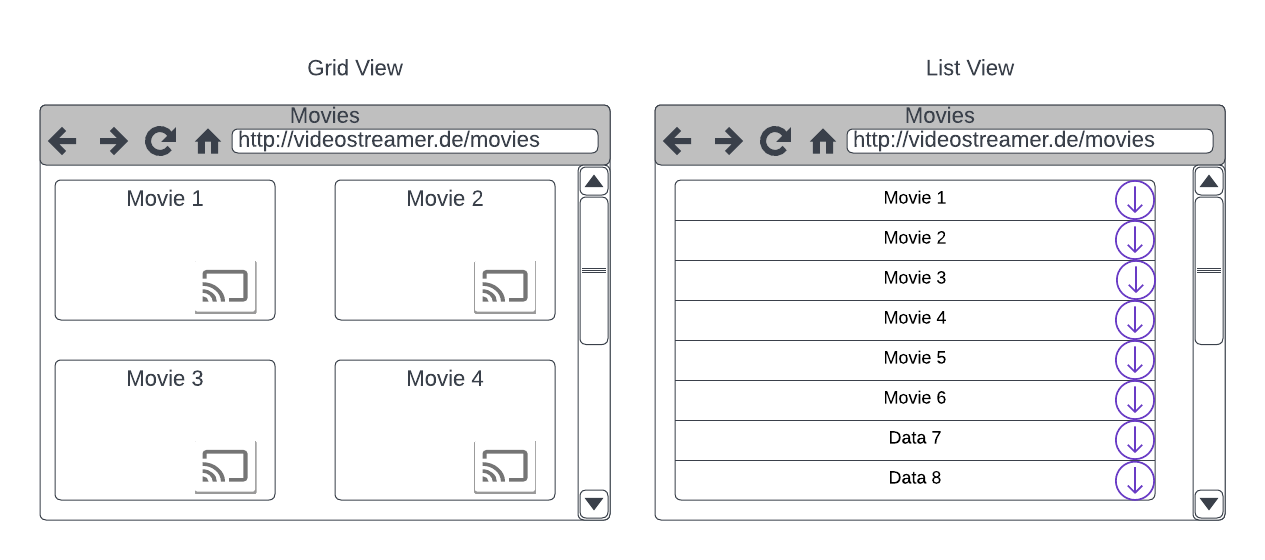
\includegraphics[width=1.0\textwidth]{images/solution-ideas/Experimentvariants.png}
	\caption{Example Experiment variants}
	\label{solutionideas:fig:experimentingvariants}
\end{figure}

\section{Measure}
\subsection{Prototypes for User Testing}
\subsection{Measuring the Experiment and Task results}
\section{Learn}
\subsection{Analysis}
\label{solutionideas:section:dataanalysis}

In our solution, we focus on data-driven development. 
To determine the ``Winner'' among the variants of a product's component, we perform data analytics on the feedback data we receive from the \texttt{Task Model} and the \texttt{Experiment Model}.
We perform the \texttt{Quantitative} (presented in section \ref{solutionideas:paragraph:quantitative}), \texttt{Qualitative} (presented in section \ref{solutionideas:paragraph:qualitative}), and the \texttt{Task} (presented in section \ref{solutionideas:paragraph:taskanalysis}) analyses of the data.

% \begin{figure}[ht]
% 	\centering
%   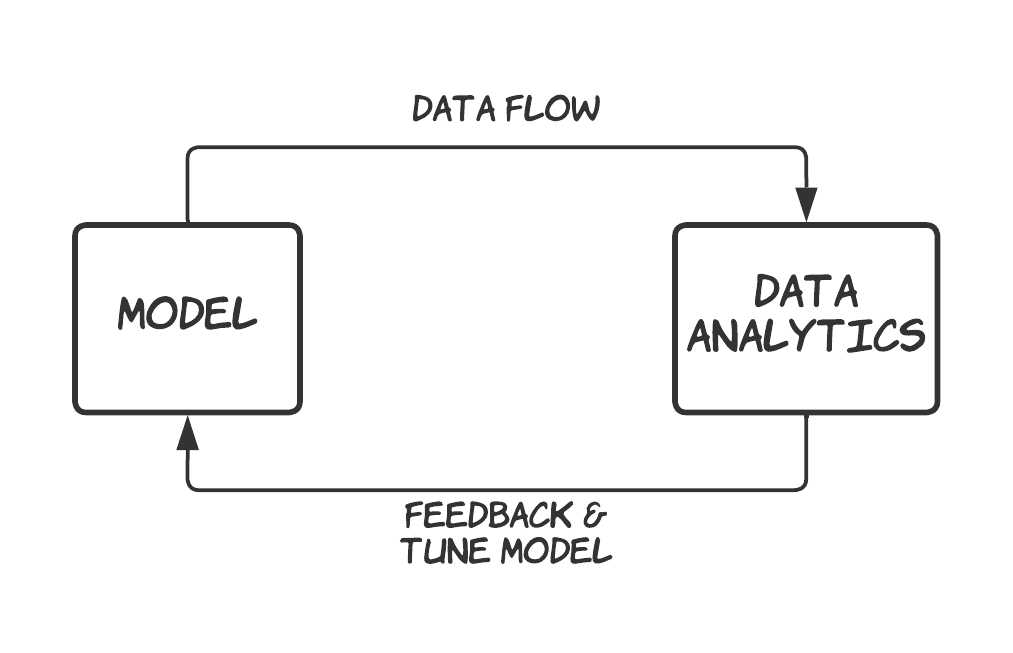
\includegraphics[width=0.5\textwidth]{images/solution-ideas/dd-development.png}
% 	\caption{Model-based \& Data Driven development}
% 	\label{solutionideas:fig:dddevelopment}
% \end{figure}

\paragraph{Quantitative Analysis:}
\label{solutionideas:paragraph:quantitative}
Quantitative analysis uses mathematical and statistical methods to determine the behavior of the data.
In quantitative research, various descriptive statistics methods like Means, Median, Variances, Standard Deviations, etc., are used to find some causal relationships in the data.

From the \texttt{Experiment Model}, we can calculate the measurements on various product components. 
(E.g., For the MoviesView component, the measurements could be ``Watch time'' to measure the duration of time spent by the user on that variant, ``Click Rate'' to count the clicks, etc.) 
Then, the experimenting server can calculate the measurements' mean (assume the mean is specified in the experiment). 
For validation, a significance test can be calculated to determine the probability of the event's occurrence, claim from the mean, and declare the winner variant.

\paragraph{Qualitative Analysis:}
\label{solutionideas:paragraph:qualitative}
To further improve, we need to perform qualitative analysis.
Qualitative analysis is used to determine the users' behavior and semantics.
Qualitative research data is usually unstructured, coming from open-ended surveys, interviews, etc. 
Our goal is to turn the unstructured data into a detailed description of the critical aspects of the problem.
In our solution, we propose to perform a qualitative analysis of the data by asking some open-ended questions to the users
(E.g., questions like ``What do you think about the Look and feel of the software application?'', ``Are the items on the page easily locatable?'', etc.).
The users' responses can be studied using some tools using the inductive or deductive coding technique. 
% If we select the inductive coding approach, we will scrutinize the reactions and those which are similar and group them. 
% These groups will be coded into labels, and we will formalize and analyze the categories. 
% To understand the process better, see figure \ref{solutionideas:fig:qualitative}. 
So, in the end, we get feedback from this process on which variants are better for the users. 
This information is forwarded to the models for modifying the prototypes.

% \begin{figure}[ht]
% 	\centering
%   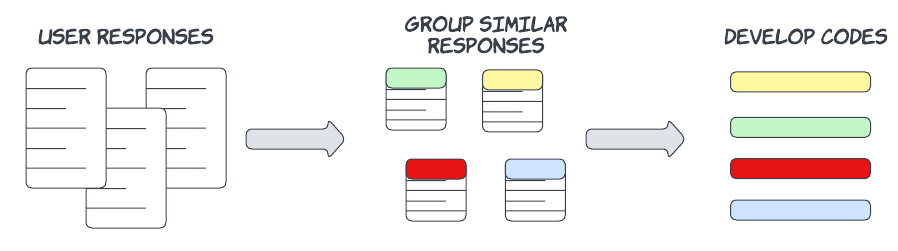
\includegraphics[width=1\textwidth]{images/solution-ideas/qualitative.png}
% 	\caption{Qualitative analysis using inductive coding}
% 	\label{solutionideas:fig:qualitative}
% \end{figure}

\paragraph{Task analysis:}
\label{solutionideas:paragraph:taskanalysis}
We also receive the data from the \texttt{Task Model}. 
Its data can be used to calculate the efficiency of the variant. A task model contains measurements for getting feedback from the users. (E.g., If the task is to locate a particular movie, we can calculate the number of clicks and time required as measurements for the users to reach their destination.
This testing type is called ``\texttt{Supervised testing}'' \cite{article:dataanalysis:supervisedtest}.
So, we observe the users, and they know the result (i.e., the movie they need to locate). 
This process gives us more accurate feedback on which variant performs better, and we can then update the prototype as per our triangle relationship (see fig \ref{solutionideas:fig:triangle}).

\subsection{Improving the Prototype}
\label{solutionideas:subsection:improvingprototypes}